\documentclass [a4paper,10pt] {article}

\usepackage{graphicx}
\usepackage{german}
\usepackage{titlesec}
\usepackage{standalone}
\usepackage{hyperref}
\usepackage[utf8]{inputenc}

\titleformat*{\section}{\LARGE \bfseries}
\titleformat*{\subsection}{\Large \bfseries}

\titlespacing*{\section}{0pt}{*4}{*2}
\titlespacing*{\subsection}{0pt}{*4}{*1.5}

\setlength{\parindent}{0pt}

\begin {document}

\begin{titlepage}
	\raggedleft
	
\includegraphics[width=5cm]{HFULogo}\par\vspace{1cm}

	\centering
	\vfill

	\LARGE FHF Train \par
	\vspace{1cm}
	
	\Large Semesterprojekt 2018 \\
	\vfill
	
	\Large Autoren: \\ 
	Stephan Mosbach AIB 6 \\
 	Ilirian Halilaj AIB6 \\ 
	Jonas Wiedle AIN6 \\ 
	Kevin Junk AIN4 \\
	Alexander Leibinger AIN6\par
	
	\vfill
	Referent: Prof. Dr. Rainer M"uller\par

	\vfill
\end{titlepage}

	\section*{Abstract}

	\vspace{5mm}

	This Project is presented by the University of Furtwangen.

\newpage

\tableofcontents

\newpage
	\section{Einleitung}
	
		Mit dieser Dokumentation wollen wir den Lesern das Vorgehen unserer Projektgruppe für das Semesterprojekt „FHFTrain“ n"aherbringen und einen Einblick in die 			
		Problematik und die daraus resultierenden Ergebnisse im Rahmen des Projektes aus einer projektorganisatorischen und einer informationstechnischen Sicht darstellen. \par
		Das Ziel unseres Projektes ist es ein Yocto Image von einem Server/Raspberry Pi über das Netzwerk automatisch auf den Zug geladen und ausgeführt werden.
	
\newpage
	\documentclass{article}
\usepackage{german}
\begin{document}
	\section{Projektbeschreibung}
Ziel dieses Projekts ist es ein eingebettetes Betriebssystem f"ur einen Raspberry Pi zu erstellen. Dieses Raspberry Pi ist bereits auf einer Modelleisenbahn montiert und soll eine Kontrolle des Zuges und die R"uckgabe von Daten erm"oglichen.
Um eventuelle Ver"anderung am Kernel zu vereinfachen, soll ein Deploykonzept entwickeln, welches die "Anderungen "uber das Netzwerk erm"oglicht. Dies soll den mechanischen Zugriff auf die SD-Karte abl"osen.
Um ein ma"sgefertigtes Linux Kernel zu erschaffen k"onnen wir das Open-Source Werkzeug Yocto benutzen. Dieses erm"oglicht es ein Linux Betriebssystem f"ur ein eingebettetes System zu gestallten. Es erm"oglicht die Architektur des CPU's selbst zu gestalten, indem man Komponenten entfernen und hinzuf"ugen kann.
Eine bereits funktionsf"ahige Anwendungssoftware die mit IBM-Rhapsody entwickelt wurde soll in den Prozess integriert werden.
\end{document}
\newpage
	\section{Zeitplan}
		\vfill
\newpage
	\author{Jonas Wiedle}
\date{09.06.2018}
\documentclass{article}
\usepackage[utf8]{inputenc}
\usepackage{helvet}
\usepackage{graphicx}
\PassOptionsToPackage{hyphens}{url}\usepackage{hyperref}
\renewcommand{\familydefault}{\sfdefault}
\begin{document}
\normalsize
\section{Netzwerkboot-und Synchronisierung}
\subsection{Einfuehrung}
Zusammen mit Alexander Leibinger, habe ich am Abschnitt 'Netzwerk' des Projekts gearbeitet. Das Ziel war das erarbeiten eines Deploykonzepts, um Änderungen und Anwendungen auf den Pi zu übertragen, ohne dabei die SD-Karte physikalisch herausnehmen zu müssen.
Hierbei gab es zwei verschiedene herangehensweisen. Die erste war der Netzwerkboot, den wir allerdings aufgrund von Problemen und Zeitmangel verwerfen mussten. Die zweite und deutlich effizientere Variante war das Synchronisieren der Dateien mithilfe des Tools rsync.
\subsection{Definition PXE-Netzwerkboot}
Der Begriff PXE steht für "Preboot Execution Environment" und beschreibt das Ausführen von XYZ vor dem Bootvorgang. Ein Gerät, welches über eine PXE-fähige Netzwerkkarte verfügt erhält vor dem eigentlichen Bootvorgang eine Konfiguration aus dem Netzwerk über DHCP. 
Dadurch bekommt das Gerät über einen TFTP-Server im Netzwerk einen Bootloader zugeschickt.  Ab hier kann man Live-Distributionen laden oder mithilfe eines NFS-Servers ein Dateisystem laden.
\subsection{Definition rsync}
Das Programm rsync ist in der Lage Dateien und Ordner lokal oder auch über das Netzwerk zu synchronisieren. Es überprüft über den Zeitstempel, wann ein Ordner oder eine Datei zuletzt geändert wurde. Sind diese am Ziel veraltet werden diese mit der aktuellen Version der Quelle überschrieben.
Es sind zudem viele weitere Optionen vorhanden mit denen man genau kontrollieren kann wie diese Synchronisation abläuft. Daher war rsync eine gute Alternative zum PXE-Netzwerkboot.
\newpage
\subsection{Ablauf (Jonas Wiedle)}
In den ersten ein bis zwei Wochen las ich mich in das Thema Netzwerkboot ein. Ich fand heraus, dass für den funktionierenden Netzwerkboot einen Server brauchte und beliebig viele Clients. Die einzige Vorraussetzung die der Client hier mitbringen muss ist, dass die Netzwerkkarte auch zum PXE-Boot fähig ist.
Auf der Serverseite wird hier ein DHCP-Server und ein TFTP-Server zur Dateiübertragung benötigt. Allerdings war mir klar, dass das Projekt am Ende im C-Labor lauffähig sein sollte. Allerdings gibt es bereits mehrere DHCP-Server im Hochschulnetz. Also suchte ich nach einer Möglichkeit den PXE-Boot zum laufen zu bekommen, ohne das der Server und die anderen DHCP-Server im Hochschulnetz sich gegenseitig Probleme bereiten würden. Ich stieß auf den Begriff  'Proxy-DHCP', welcher am Ablauf des des PXE-Boot nur in soweit etwas verändert, dass sich der Server problemlos in ein Netz mit bereits verfügbaren DHCP-Server eingliedert. Der Proxy-DHCP-Server übernimmt nur die Anfragen der Clients die direkt den PXE-Boot betreffen. 
\\\\
Beim zweiten Treffen bekamen wir den ersten der beiden Raspberry Pi's 3 damit wir mit dem Arbeiten beginnen konnten. Im gegensatz zu älteren Modellen sind die Raspberry Pi der Version 3 ohne Probleme zum Netzwerkboot fähig. Von Seiten der Zeiteinteilung aus, wollten wir es schaffen nach zwei Wochen den PI zum booten zu bekommen.
Zuerst sprachen wir mit dem Labor-Administrator und ließen dem Pi eine feste IP-Adresse zuweisen, was das Arbeiten vereinfacht. Herr Müller hatte uns gegenüber erwähnt, dass es im Labor bereits einen TFTP-Server gäbe den wir eventuell nutzen könnten. Herr Neubeck sagte uns allerdings, dass wir nicht direkt auf dem TFTP-Server arbeiten dürften.
Sollten wir allerdings die richtige Konfiguration kennen, würde er es für uns auf dem Server einstellen.
Jedoch mussten wir in der Lage sein den Netzwerkboot zu testen um diesen richtig konfigurieren zu können. Herr Müller übergab uns in Folge dessen beim nächsten Treffen einen älteren Raspberry, damit wir zwischen den zwei Pi's eine Testumgebung aufbauen könnten. Hierbei würde ein Pi den Server darstellen und der andere den Client.
Ein bis zwei Tage später bekamen wir auch noch den neueren Pi, somit hatten wir zwei Raspberry Pi 3. Bis zum nächsten Treffen sollte der Netzwerkboot funktionieren, was allerdings problematisch war. in dieser Zeit war ich sehr oft an der Hochschule und arbeitete auch öfters Zuhause um das Booten zum laufen zu bekommen, allerdings ohne großen Erfolg, dazu später mehr.
\\\\
Ich testete den Netzwerkboot auch zwischen zwei virtuellen Maschinen, wo er einandfrei funktionierte. Allerdings war mir und auch Alexander beim Boot des Pi's kein Erfolg vergönnt. Vor dem nächsten Treffen schrieb ich auch eine E-Mail an Herr Müller, welcher mir ebenfalls zwei Links für Anleitungen schickte. 
Eine der Anleitungen hatte ich jedoch bereits ausprobiert und die andere funktionierte ebenfalls nicht. Er machte mich darauf aufmerksam, dass die bootcode.bin Datei für den initiellen Boot auf der SD-Karte vorhanden sein müsste. 
\\\\ 
Das war allerdings sehr widersprüchlich, da viele Anleitungen für den Raspberry Pi diese Datei nie erwähnten und laut Benutzerberichten zufolge be dneren der netzwerkboot auch ohne jegliche Datei auf der SD-Karte funktionierte. Zudem las ich auch einen Artikel, welcher darauf hinwieß, dass die älteren Pi's zwar diese Datei benötigt hätten, der Raspberry Pi 3 allerdings ohne in der Lage ist den Netzwerboot erfolgreich zu initiieren.
\\\\
Beim nächsten Treffen einigten wir uns darauf, es mit der Datei auf der SD-Karte zu versuchen, was Alexander ausprobierte. Wir hatten jedoch beide keine positiven Erfolge. Ich hatte mich seit längerem bereits nach einer Alternative umgesehn, da wir bereits seh viel zeit in den netzwerboot investiert hatten und dieser immer noch nicht funkktionierte.
Mein erster Gedanke war rsync, ein Backuptool mit welchem ich auch schon öfters in der Hochschulzeit und während meines Praxissemesters gearbeitet hatte. Beim Projekttreffen einigten wir uns darauf das Thema Netzwerkboot ruhen zu lassen und es mit rsync zu versuchen.
Für rsync benötigten wir einen Ordner auf dem Server von welchem wir das Dateisystem auf den Pi synchronisieren könnten, Herr Müller erstellte uns hierzu den Ordner ss18 FHFTrain im projects Ordner. Den ersten Prototyp des rsync Skripts schrieb ich über die Ferien in Java. Ich entschied mich jedoch dazu es in ein Skript umzuwandeln, da dies kleiner übersichtlicher und einfacher wäre in einen Service umzuwandeln. Den ersten Prototypen testete ich auch zuhause zwischen meinen beiden VMs. Der Service aktivierte sich automatisch beim hochfahren und synchronisierte Ordner in der lokalen VM.
Vom nächsten Treffen an wollten wir, dass rsync im Labor funktionierte, zudem kam der Wunsch von Stephan auf, dass Dateien die nicht mehr auf derm Server vorhanden wären auch lokal gelöscht werden sollten. Das sei aus dem Grund, da bei Änderungen auf dem Server eventuell alte Dateien entstehen könnten, welche im Betriebssystem zu problemen führen könnten, falls diese nicht gelöscht werden sollten. Ich hinterlegte das Skript, sowie den Service auf dem Raspberry Pi und erstellte einen SSH-Key, damit der Service sich beim hochfahren automatisch beim Server anmelden und sich die Dateien ziehen kann.
\\\\
Nach dem nächsten Treffen wollten wir uns von Herr Neubeck einen Benutzer erstellen lassen, damit wir uns nicht über unsere privaten Benutzer authentifizieren müssten was ebenfalls ein Sicherheitsrisiko darstellte.
Herr Neubeck schlug uns allerding vor auf dem Pi über fstab ein NFS zu mounten. Dadurch bräuchten wir keine authentifizierung und müssten das Skript nur geringfügig abändern. Kevin lud uns das Root-File-System auf den Server in unseren Ordner hoch.
Ab hier wurde es etwas komplizierter, da wir nicht nur einen Ordner sondern ein gesamtes Betriebssystem auf einmal synchronisierten. Mit der zusätzlichen Option des löschens kann viel schief gehen. Alexander und ich vertan uns beim ersten Befehl etwas und löschten das System vom Raspberry Pi, was Alexander allerdings wieder aufspielen konnte.
\\\\\\
Später Zuhause konnte ich den Befehl allerdings perfektionieren, er synchronisierte und löschte daten, allerdings funktionierte das gesamte System noch nach erneutem hochfahren und alle Ordner waren synchronisiert.
Zurück in der Hochschule gelang es uns den Ordner über das Netzwerk per NFS zu mounten. Nun fehlt es uns nur noch den neuen Befehl auszutesten. Hierbei muss ich darauf achten, den lokalen NFS Ordner von der Synchronisierung auszuschließen, da sonst ein Problem durch eine Schleife oder ähnliches entstehen könnte.
\subsection{Versuche und Probleme (Jonas Wiedle)}

Timer Service und Internet

\subsection{rsync-Synchronisierung}
Wie bereits vorher erwähnt, schrieb ich das erste rsync-Programm in den Pfingstferien. Zuerst schrieb ich es in Java, änderte es jedoch dann in ein Bash-Skript ab, da dies übersichtlicher ist und einfacher als Service zu implementieren ist.
Das Bild unten zeigt die erste Version, die ich in Java geschrieben habe:
\\\\
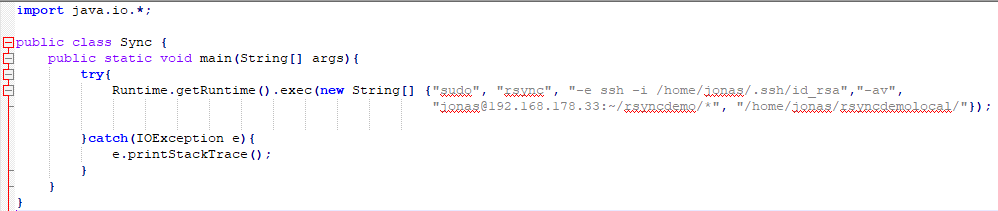
\includegraphics[width=1.0\textwidth]{JavaPrototype.png}
\\\\
Ich testete das Java-Programm zwischen meinen VMs was erfolgreich funktionierte. Ich änderte es jedoch aufgrund der oben gennanten Gründe in das unten gezeigte Bash-Skript ab. Ich synchronisierte anfangs zum Test nur einzelne Ordner und kein Dateisystem.
\\\\
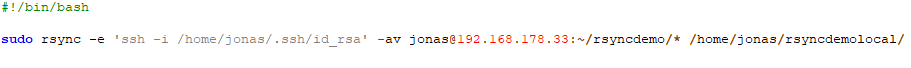
\includegraphics[width=1.0\textwidth]{syncmasterv1.png}
\\\\
Alexander passte das Bash-Skript dann so an, dass es im Labor laufen würde. Schließlich sollte es in der Lage sein mit dem Dateisystem vom Server das eigene, lokale zu Überschreiben.
Nach dem Test, bei welchem das Betriebssystem gelöscht wurde, wollte ich den Befehl am selben Tag noch fertigstellen. Diesesmal machte ich den Volltest mit kopieren und überschreiben des lokalen Dateisystems.
Der Befehl konnte noch nicht zwischen dem Pi und dem Server getestet werden, ist allerdings soweit es die VMs angeht funktionstüchtig:
\\\\
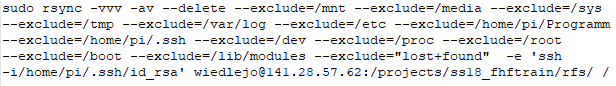
\includegraphics[width=1.0\textwidth]{skriptv3.png}
\\\\
\begin{itemize}  
\item Wir benutzen \textbf{sudo} damit der Befehl ohne Probleme ausgeführt werden kann. Da der Befehl viele Dateien überschreibt und auch löscht ist dieser Parameter vonnöten.
\item Danach wird \textbf{rsync} selbst aufgerufen
\item Die Option \textbf{-v}, gibt den Ablauf des Programms auf der Konsole aus. Da wir allerdings Fehler, die auftauchen könnten genau Untersuchen möchten, benutzen wir die Option \textbf{-vvv}, für maximale Ausgabe.
\item \textbf{Beschreibung muss noch fertig werden}
\end{itemize}

Rsync-Beschreibung  muss noch zur finalen 

Die erste Version des Services, den ich zuhause erstellte sah folgendermaßen aus:
\\\\
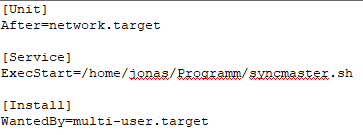
\includegraphics[width=1.0\textwidth]{servicev1.png}
Damit dieser auch an der Hochschule funktionierte musste ich allerdings ein paar Dinge ändern:
\\\\
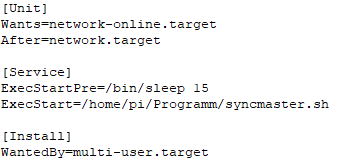
\includegraphics[width=1.0\textwidth]{servicev2.png}

Aufbau des Service:
\begin{itemize}  
\item Mit \textbf{Wants}-und \textbf{After=network-online.target} lege ich fest, dass der Service erst starten soll, wenn der Pi ein bestehende Netzwerkverbindung hat.
\item Da der Service zum Teil dennoch zu früh gestartet hat, benutze ich \textbf{ExecStartPre=/bin/sleep/ 15}, was den Service erst starten lässt nachdem 15 Sekunden abgelaufen sind.
\item \textbf{ExecStart=/home/pi/Programm/syncmaster.sh} startet dann das eigentliche Skript indem es im Programm Ordner aufgerufen wird.
\item Der Abschnitt \textbf{[Install]} legt fest wann der Service oder die Unit gestartet wird. 
\item Der Befehl \textbf{WantedBy=multi-user.target} legt fest, dass der Service startet, sobald das System hochfährt oder neugestartet wird.
\end{itemize}

fstab-Beschreibung:
\begin{itemize}
\item \textbf{fstab screenshot + aufbau}
\end{itemize}
\end{document}
\newpage
	\documentclass[a4paper,10pt] {article}
\begin {document}
	\section{Netzwerkboot}	
		
		Um das Projekt zu realisieren wurde das Team in Mehrere Gruppen aufgeteilt. Jonas und Alexander versuchten den Netzwerkboot umzusetzen.
		
		Beim Netzwerkboot war das Ziel, dass der Pi 3 der im Zug verbaut ist, beim Start nicht über die SD Karte oder ein anderes angeschlossenes Speichergerät Startet, sondern über ein Betriebssystem Image das auf einem DHCP/TFTP Server liegt.
		Der große Vorteile hierbei ist, dass es künftig keine Probleme mehr mit kaputten SD Karten gibt.
		
		In ersten Tests richteten wir eine Pi 3 VM auf dem PC ein. Diese diente als Server einen Pi 3 den wir zur Verfügung hatten richteten wir als Client ein. 
		
		\subsection{Client Konfiguration}
		
			Der Client muss zuerst mithilfe einer SD Card gebootet werden. Mit dem Befehl
			
				echo program\_usb\_boot\_mode=1 | sudo tee -a /boot/config.txt
			
			schalten wir den USB boot mode ein. Um zu überprüfen ob der OTP Speicher im Pi nun richtig konfiguriert ist, starten wir den Pi neu und führen den Befehl
			
				vcgencmd otp\_dump | grep 17:
			
			aus. Die Ausgabe muss 0x3020000a sein. Falls die Ausgabe Korrekt ist, entfernen wir nun wieder den Eintrag in der config.txt. Der Client ist nun Konfiguriert. 
			
		\vfill
		
		\subsection{Server Konfiguration}
		
			Bei der Server Konfiguration erweitern wir das Filesystem auf die komplette SD Karte mit dem Konfigurationstool 
			
			sudo raspi-config
			
			Da der Client ein root filesystem benötigt zum booten, Erstellen wir ein Abbild des aktuellen Filesystem und hinterlegen es im Verzeichniss /nfs/client1.
			 
			sudo mkdir -p /nfs/client1
			sudo rsync -xa --progress --exclude /nfs / /nfs/client1
			
			Nun müssen die SSH Schlüssel erneuert werden
			
			cd /nfs/client1
			sudo mount --bind /dev dev
			sudo mount --bind /sys sys
			sudo mount --bind /proc proc
			sudo chroot .
			rm /etc/ssh/ssh\_host\_*
			dpkg-reconfigure openssh-server
			exit
			sudo umount dev
			sudo umount sys
			sudo umount proc
			
			wir benötigen nun noch die Netzwerkinformationen. Hierzu muss der Pi mit dem Netzwerk verbunden sein.
			
			ip route | grep default | awk '{print \$3}'
			ip -4 addr show dev eth0 | grep inet
			
			Die Ausgabe sollte so aussehen
			
			inet 192.168.1.101/24 brd 192.168.1.255 scope global eth0
			
			Server IP Adresse: 192.168.1.101
			Brodcast Adresse: 192.168.1.255
			eth0: Verbindung über LAN Kabel
			
			die IP Adresse vom DNS Server bekommen wir mit 
			
			cat /etc/resolv.conf
			
			der Pi selber benötigt noch eine Statische IP Adresse
			
			sudo nano /etc/network/Interfaces
			
			Hier die Zeile 
			
			iface eth0 inet manual 
			
			ersetzen mit 
			
			auto eth0
			iface eth0 inet static 
				address 192.168.1.2
				netmask 255.255.255.0
				gateway 192.168.1.1
				
			Die gateway Adresse ist die Adresse die wir aus resolv.conf ausgelesen haben
			
			den DHCP client Daemon müssen wir auch noch ausschalten
			
			sudo systemctl disable dhcpcd
			sudo systemctl enable Networking
			
			sudo reboot
			
			Mit dem Neustart wurden unsere Änderungen übernommen. Wir haben nun kein funktionierendes DNS mehr. Wir fügen nun unsere Server Konfiguration ein. nameserver entspricht der gateway Adresse.
			 
			echo "nameserver 192.168.1.1" | sudo tee /etc/resolv.conf
			
			die Datei darf durch dnsmasq nicht mehr verändert werden weshalb wir sie mit dem Befehl
			
			sudo chattr +i /etc/resolv.conf
			
			unveränderbar machen. Es ist nun zwingend erforderlich zusätzliche Software zu installieren 
			
			sudo apt-get update
			sudo apt-get install dnsmasq tcpdump
			
			Mit dem nächsten Befehl stoppen wir die DNS Namensauflösung mit dnsmasq 
			
			sudo rm /etc/resolvconf/update.d/dnsmasq
			sudo reboot
			
			Wir starten nun tcpdump um nach DHCP Paketen vom Client Raspberry Pi zu suchen
			
			sudo tcpdump -i eth0 port bootpc
						
		\vfill
		
		\subsection{Inbetriebnahme}
			
			Nachdem nun auch die Netzwerk config abgeschlossen ist schließen wir den Client Raspberry ans Netzwerk an und starten ihn. Nach 10 Sekunden sollten wir auf dem Client beobachten können, dass die LED anfängt zu leuchten. Auf dem Bildschirm sollten wir nun Pakete mit der Bezeichnung BOOTP/DHCP, Request bekommen.
			
			IP 0.0.0.0.bootpc > 255.255.255.255.bootps: BOOTP/DHCP, Request from b8:27:eb...
		
			Der Server empfängt nun Anfragen vom Client kann aber noch nicht Antworten. Hierfür müssen wir erst noch dnsmasq konfigurieren
			
			echo | sudo tee /etc/dnsmasq.conf
			sudo nano /etc/dnsmasq.conf
			
			Den gesamten Inhalt der Datei ersetzen durch
			
			port=0
			dhcp-range=192.168.1.255,proxy
			log-dhcp
			enable-tftp
			tftp-root=/tftpboot
			pxe-service=0,``Raspberry Pi Boot''
			
			dhcp-range = Brodcast Adresse
			
			Das Verzeichniss /tftboot müssen wir noch erstellen
			
			sudo mkdir /tftpboot
			sudo chmod 777 /tftpboot
			sudo systemctl enable dnsmasq.service
			sudo systemctl restart dnsmasq.service
			
			Wir überwachen jetzt das dnsmasq Protokoll mit 
			
			tail -F /var/log/daemon.log
			
			und suchen dort einen Einträgen die ungefähr so aussehen
			
			raspberrypi dnsmasq-tftp[1903]: file /tftpboot/bootcode.bin not found
			
			wir holen uns nun die Datei bootcode.bin und start.elf in unser /tftboot Verzeichniss indem wir das komplette boot Verzeichnis kopieren
			
			cp -r /boot/* /tftpboot
			sudo systemctl restart dnsmasq
			
			Für einen ersten Test verwendeten wir nun das am Anfang kopierte root filesystem in /nfs/client1 dieses sollte später durch unser in Yocto erstelltes root filesystem ersetzt werden
			
			sudo apt-get install nfs-kernel-server
			echo ``/nfs/client1 *(rw,sync,no\_subtree\_check,no\_root\_squash)'' | sudo tee -a /etc/exports
			sudo systemctl enable rpcbind
			sudo systemctl restart rpcbind
			sudo systemctl enable nfs-kernel-server
			sudo systemctl restart nfs-kernel-server
			
			/tftpboot/cmdline.txt muss nun noch angepasst werden
			
			root=/dev/nfs nfsroot=192.168.1.2:/nfs/client1 rw ip=dhcp rootwait elevator=deadline
			
			Die IP Adresse entspricht der vom Client. Abschließend müssen noch die SD Karten Einträge in fstab gelöscht werden
			
			sudo nano /nfs/client1/etc/fstab
			
			Hier die Einträge 
			
			/dev/mmcblkp1
			/dev/mmcblkp2
			
			löschen. Nun sollte der Netzwerkboot richtig konfiguriert sein.
			
		\vfill
		
		\subsection{rsync}
			Leider funktionierte der Netzwerkboot nicht. Wir haben im Internet noch diverse andere Anleitungen ausprobiert aber alle ohne Erfolg. In einem Versuch hatten wir das System soweit, dass sich der Client ein Paket vom Server holte, danach aber aufhörte. Als Alternative zum Netzwerkboot hinterlegten wir nun ein root filesystem auf dem Server im Labor im Verzeichnis /projects/ss18\_fhftrain/rfs. Dieses ist erreichbar über 
			
			Server:141.28.57.62 
			Port: 12345
			
			Das root filesystem ist mithilfe von Yocto erstellt worden und läuft auch auf dem Pi. Mithilfe von rsync übernimmt der Pi beim Einschalten alle Änderungen die im Verzeichnis /projects/ss18\_fhftrain/rfs gemacht wurden. 
			
			Als erstes muss rsync installiert werden
			
			sudo apt-get install rsync 
			
			Die Syntax des rsync Befehls sieht folgendermaßen aus
			
			rsync [OPTIONEN] QUELLE(N) ZIEL 
			
			Quelle: /projects/ss18\_fhftrain/rfs/
			Ziel: /
			
			Optionen:
			Es ist wichtig einige Pfade und Ordner zu excludieren. Diese enthalten unter anderem Hardware spezifische Daten die nicht überschrieben werden dürfen. Das Verzeichnis mit dem rsync Befehl müssen wir auch excludieren. 
			
			--exclude=/mnt 
			--exclude=/media 
			--exclude=/sys 
			--exclude=/tmp 
			--exclude=/var/log 
			--exclude=/etc 
			--exclude=/dev 
			--exclude=/proc 
			--exclude=/root 
			--exclude=/boot 
			--exclude=/lib/modules 
			--exclude=``lost+found''
			
			--exclude=/home/pi/Programm 
			--exclude=/home/pi/.ssh 
			
			Andere Optionen:
			
			-vvv
			gibt uns während des Synchronisierens Debuginfos aller ausgeführter Schritte aus 
			
			-av
			
			--delete
			vergleicht Quellverzeichnisse und Zielverzeichnisse und sorgt dafür, dass Dateien, die im Quellverzeichnis nicht (mehr) vorhanden sind, im Zielverzeichnis gelöscht werden			
		
		\vfill
		
\newpage

\end {document}



\newpage
	\documentclass[a4paper,10pt] {article}
\usepackage{graphicx}
\begin {document}
\section{Yocto Image}
\subsection{Einführung}

	Kevin und Stephan haben während diesem Projekt das Thema Yocto Image bearbeitet. Dabei sollten wir mit Hilfe von Yocto ein Image erstellen, welches eine Linux Distribution und die, von 
	vorherigen Gruppen erstellte, Anwendungssoftware des FHF-Trains.
	Allerdings hat die Linux Distribution wegen des Linux Kerns nicht funktioniert, weshalb wir uns dafür entschieden haben, nur ein RootFile-System mit der Anwendungssoftware zu erstellen,
	welche dann auf den FHF-Train übertragen wird.

\subsection{Definition Yocto}

	Das Yocto Projekt ist ein Open Source Werkzeug, welches für Entwickler von embedded Linux Systeme geschaffen wurde. Das Ziel von Yocto ist es, durch Einfügen und Ausschliessen
	gewählter Komponenten ein Linux System zu erstellen, welches von dem Nutzer auf das Endgerät angepasst wird. Um das alles zu ermöglichen, benutzt Yocto hauptsächlich BitBake und
	Open Embedded. Dafür haben wir Poky verwendet, welches uns ermöglicht den Kern, den bootloader und ein RootFile-System zu erstellen.
	
\subsection{Definition BitBake}
	
	BitBake ist ein Tool, welches in Metadaten gegebene Aufgaben ausführt. Diese Metadaten werden in BitBake-spezifischen Dateien gespeichert. Dazu gehören Rezepte (.bb),
	Konfigurationsdateien (.conf), Klassen (.bbclass) und Append Dateien (.bbappend). Append Dateien erweitern Rezepte, die den gleichen Namen besitzen. Diese Dateien werden in
	'layer.conf'-Dateien aufgelistet und werde durch eine 'bblayers.conf' an  BitBake referenziert.

	Es gibt verschiedene BitBake Befehle, die einem erlauben, aus den oben genannten Dateien ein Image zu erstellen. Dazu gehören:
	\begin{itemize}
	\item core-image-minimal: Das kleinste mögliche Image, welches dem Zielsystem erlaubt die Kommandozeile zu booten.
	\item core-image-base: Ein Image, welches core-image-minimal durch Hardwareunterstützung wie beispielsweise W-LAN und Bluetooth erweitert.
	\item core-image-full-cmdline: Dieses Image erweitert minimal durch Kommandozeilen-Befehle.
	\end{itemize}

\subsection{OpenEmbedded}
	Open Embedded ist eine atomatisiertes build Framework und eine Cross-Compiling Umgebung. Diese Umgebung ermöglicht es Maßgeschneiderte Linux Images für eingebettete Systeme 
	zu erstellen.
	\\ \textbf {muss noch weiter erläutert werden}
	\newpage

\subsection{Hob}
	Hob ist ein BitBake User Interface, welches das Erstellen der Images vereinfacht. Über Hob kann man einfach das Zielsystem und den BitBake-Befehl auswählen. Wenn man eine eigene
	Layer-Datei erstellt hat, kann man diese auch der Liste der aktuellen Layers hinzufügen. Des Weiteren bietet Hob eine komplette Liste von Paketen, die in den Layers aufgeführt sind 
	und lässt den User auswählen, welche er installieren möchte. Nach den Einstellung startet Hob den BitBake-Befehl und erstellt eine Image Datei.

\section{Ablauf Yocto}
\subsection{Erstellung einer virtuellen Maschine}
Um Yocto benutzen zu können mussten wir zur aller erst eine virtuelle Linux Maschine erstellen Yocto nur auf einem Linux basierten Betriebssystem funktioniert. Die folgenden Betriebssysteme wurden von den Entwicklern getestet und als stabil bezeichnet:
	\begin{itemize}
	\item Ubuntu 12.04 (LTS)
	\item Ubuntu 13.10
	\item Ubuntu 14.04 (LTS)
	\item Fedora release 19 (Schrödinger's Cat)
	\item Fedora release 20 (Heisenbug)
	\item CentOS release 6.4
	\item CentOS release 6.5
	\item Debian GNU/Linux 7.x (Wheezy)
	\item OpenSUSE 12.2
	\end{itemize}
Da wir mit Ubuntu bis jetzt am meisten Erfahrung hatten, haben wir uns recht schnell dafür entschieden Ubuntu 14.04 (LTS) zu benutzen.

\newpage
\subsection{Yocto Installation}

Sobald wir mit der Erstellung einer virtuellen Maschine fertig waren mussten wir uns um die Installation vom Yocto Projekt kümmern.
Um Yocto (bzw. Poky) zu installieren mussten wir zuerst die folgenden Pakete mittels der Kommandozeile „apt-get install“ installieren:
	\begin{itemize}
	\item gawk 
	\item wget 
	\item git-core 
	\item diffstat 
	\item unzip 
	\item texinfo 
	\item gcc-multilib 
	\item build-essential 
	\item chrpath 
	\item socat 
	\item cpio 
	\item python 
	\item python3 
	\item python3-pip
	\item python3-pexpect 
	\item xz-utils 
	\item debianutils 
	\item iputils-ping 
	\item libsdl1.2-dev 
	\item xterm
	\end{itemize}
Danach haben wir im Homeverzeichnis einen „Yocto“ Ordner angelegt indem wir mittels der Kommandozeile „git clone git://git.yoctoproject.org/poky --branch daisy“ den source Code vom Yocto Projekt heruntergeladen haben.


\subsection{Erstellung eines einfachen Images}
Mit Hilfe der Kommandozeile 'source poky/oe-init-build-env' wird es schließlich möglich Poky zu benutzen. Poky benutzt 'BitBake' um aus 'Rezpeten', Images zu machen. Bitbake ist im Grunde genommen ein Make Werkzeug das andere Make Werkzeuge (wie die, die wir ganz am Anfang installiert haben) benutzt um das Image zu bauen. 
Wir haben uns entschieden zuerst ein einfaches Image zu bauen mit Hilfe vom core-image-minimal Rezept. Dieses baut ein einfaches und leeres Root Filesystem, das eigentlich zum Testen und entwickeln von Kernels und Bootloaders gedacht ist. Um dies zu bewerkstelligen haben wir die Kommandozeile 'bitbake core-image-minimal' benutzt.
Da wir den BitBake allerdings auf einer virtuellen Maschine und nicht auf einem nativen Linux Betriebssystem haben laufen lassen hat er um die 12 Stunden gedauert (auf einem nativen Betriebssystem soll der BitBake zwischen 3 und 4 Stunden dauern).
Als das Image gebaut war konnten wir es mit Hilfe von der Kommandozeile 'runqemu qemux86' emulieren.

\subsection{Erstellung eines Root Filesystems mit Hob}
Poky bietet ein graphisches User Interface namens „Hob“ an das den BitBake Prozess übersichtlicher für den Benutzer macht:
\\\\
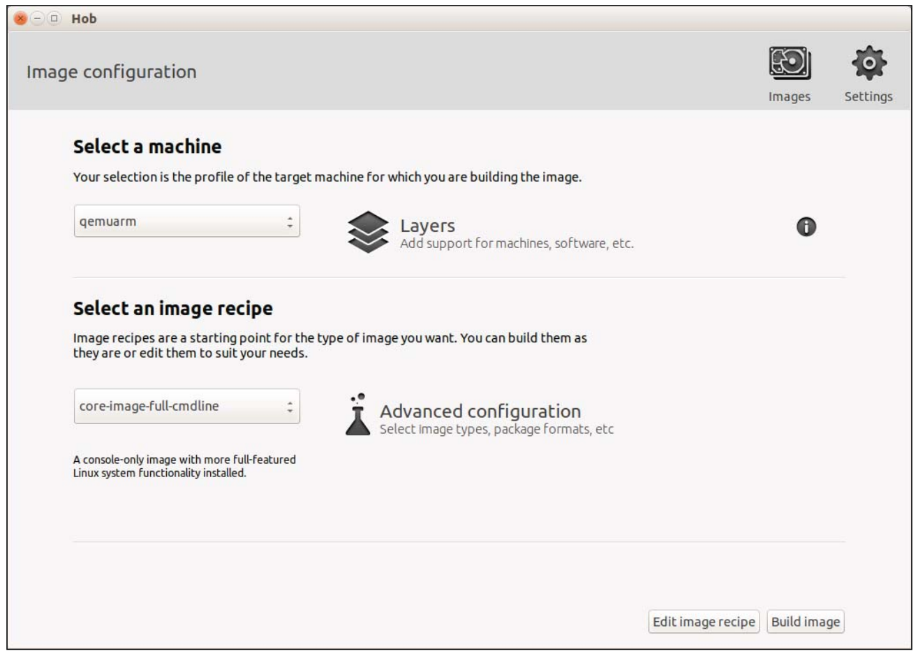
\includegraphics[width=1.0\textwidth]{Hob_Interface}
\\
\newpage
Mit Hilfe von Hob kann man dann ganz einfach eine ziel Maschine und ein Rezept aussuchen.
\\\\
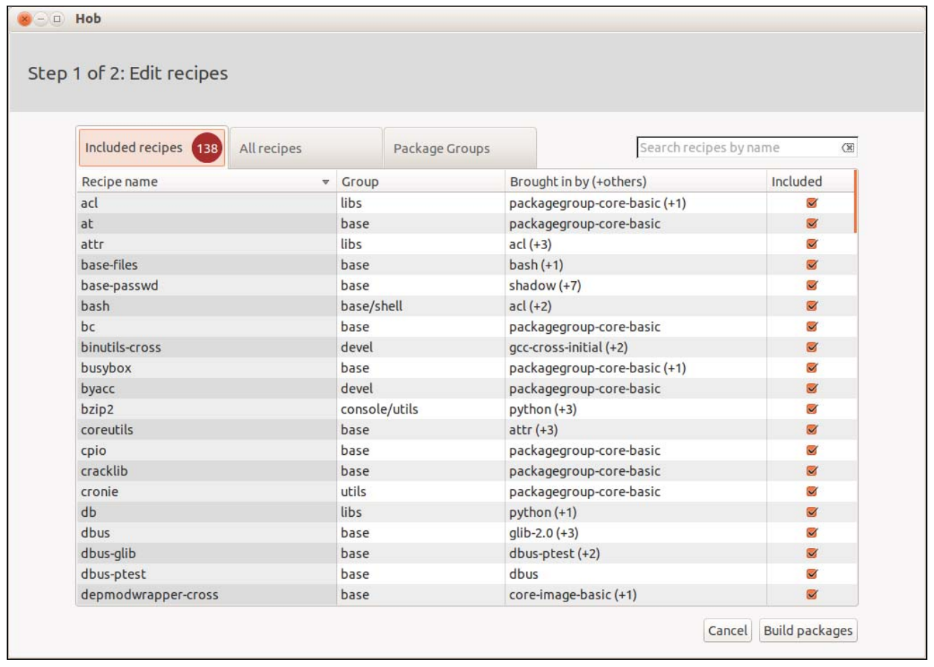
\includegraphics[width=1.0\textwidth]{Hob_Package_1}
\\\\
Danach kann man sogar wählen welche Pakete das Image braucht und welche nicht.
\\\\
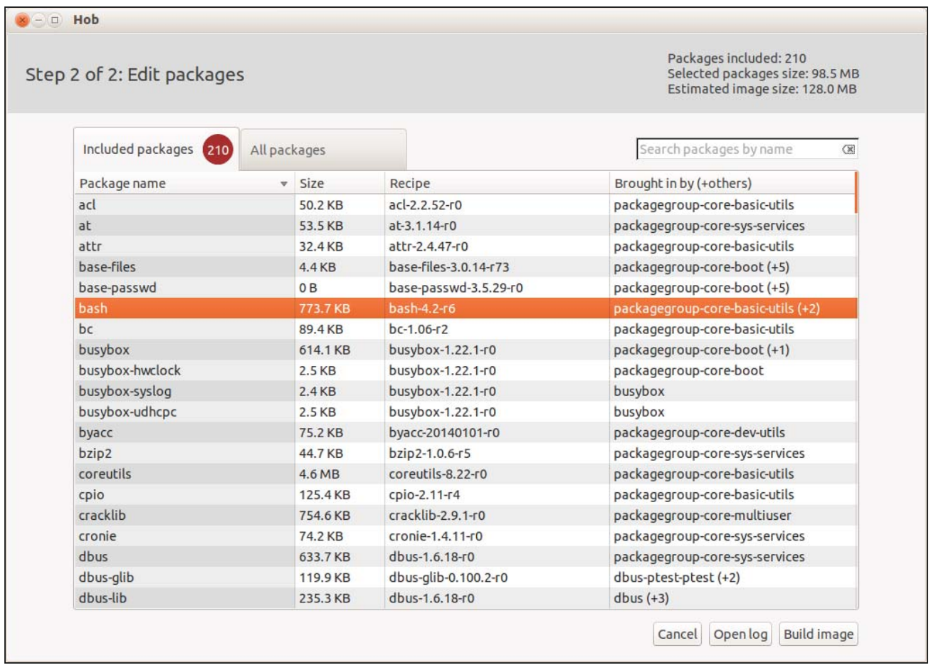
\includegraphics[width=1.0\textwidth]{Hob_Package_2}
\\\\
Nach dem auswählen der Pakete kann der Build des Images beginnen.
\\\\
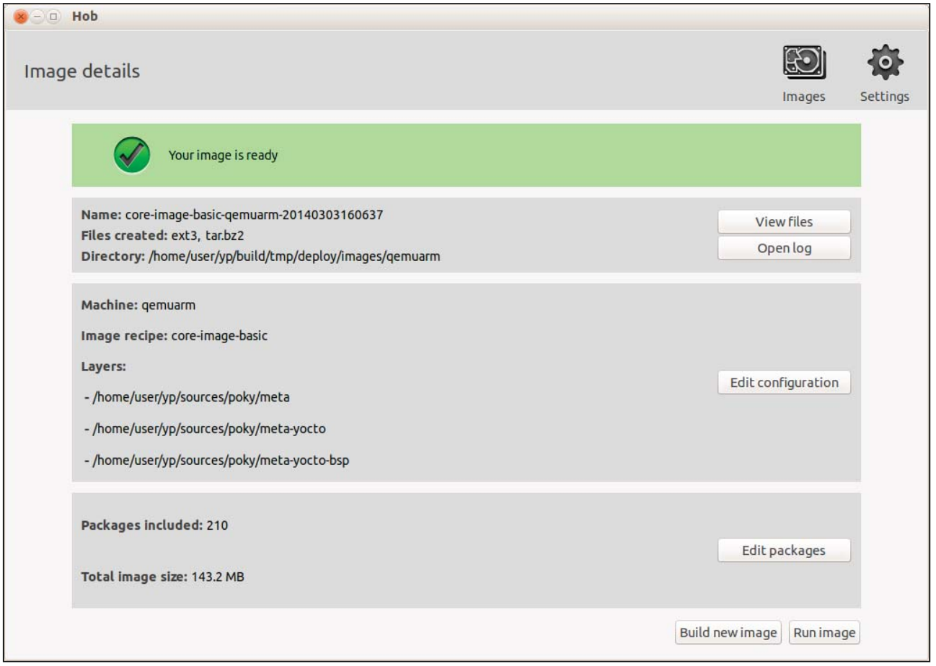
\includegraphics[width=1.0\textwidth]{Hob_Finished}
\\\\
Wenn der Build dann zu Ende ist kann das Image emuliert werden:
\\\\
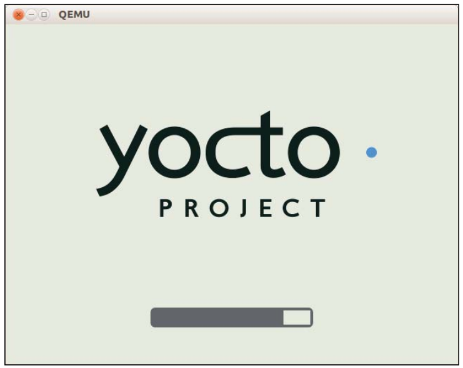
\includegraphics[width=1.0\textwidth]{Yocto_Emule}

\end {document}	


\newpage
	\begin{document}
\section{Quellenverzeichnis}
\subsection{Quellen von Jonas}
\begin{itemize}
\item \url{https://wiki.ubuntuusers.de/rsync/}\\
\item \url{https://wiki.ubuntuusers.de/systemd/Service_Units/}\\
\item \url{https://wiki.ubuntuusers.de/systemd/Units/}\\
\item \url{https://unix.stackexchange.com/questions/399830/how-can-i-define-a-systemd-target-to-start-on-boot-or-after-another-target}\\
\item \url{https://ubuntuforums.org/showthread.php?t=238672}\\
\item \url{https://www.raspberrypi.org/forums/viewtopic.php?t=156830}\\
\item \url{https://www.kernel.org/doc/Documentation/filesystems/nfs/nfsroot.txt}\\

Muss noch Quellen noch fertig hinzufügen
\end{itemize}
\end{document}
\end {document}


